%% Annexes
\chapter{Diagramme de Gantt}
% OBLIGATOIRE (consignes Pompidor) : vue synthétique de la chronologie de l'alternance.
% ----------------------------------------------------------------------------
% À ADAPTER : renomme les tâches et ajuste {début}{durée} (en MOIS depuis sept. 2024).
% \gbar{ligne}{mois de début}{durée en mois}{couleur}{libellé}
% ----------------------------------------------------------------------------
\definecolor{ganttA}{RGB}{60,120,200}
\definecolor{ganttB}{RGB}{220,120,40}
\definecolor{ganttC}{RGB}{60,160,90}

\newcommand{\gbar}[5]{%
  \fill[#4,rounded corners=2pt] (#2,{-#1+0.30}) rectangle (#2+#3,{-#1-0.30});
  \node[anchor=east,font=\footnotesize] at (-0.4,-#1) {#5};
}

\begin{figure}[H]
\centering
\resizebox{\textwidth}{!}{%
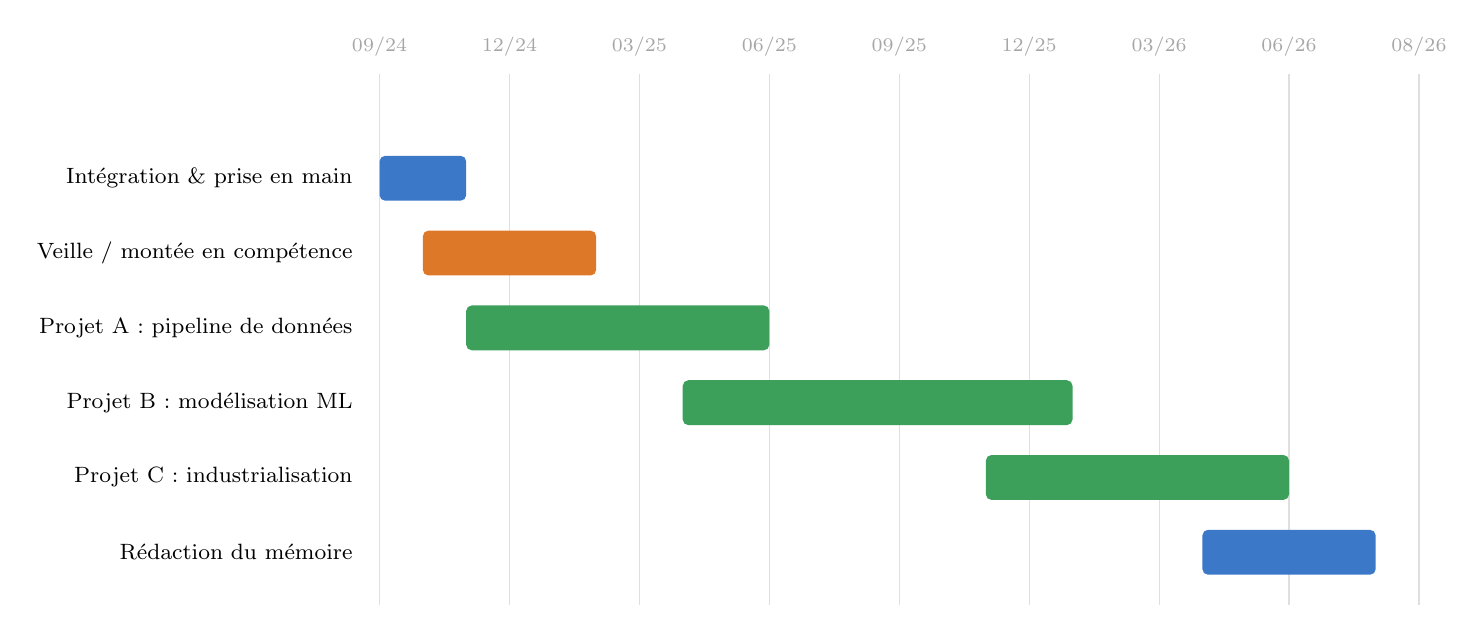
\begin{tikzpicture}[x=0.55cm,y=0.95cm]
  % --- Axe du temps : 24 mois, repères trimestriels ---
  \foreach \m/\lab in {0/{09/24},3/{12/24},6/{03/25},9/{06/25},12/{09/25},%
                       15/{12/25},18/{03/26},21/{06/26},24/{08/26}} {
    \draw[gray!25] (\m,0.4) -- (\m,-6.7);
    \node[font=\scriptsize,gray!70,anchor=south] at (\m,0.5) {\lab};
  }
  % --- Tâches (PLACEHOLDERS — à remplacer par tes vrais projets) ---
  \gbar{1}{0}{2}{ganttA}{Intégration \& prise en main}
  \gbar{2}{1}{4}{ganttB}{Veille / montée en compétence}
  \gbar{3}{2}{7}{ganttC}{Projet A : pipeline de données}
  \gbar{4}{7}{9}{ganttC}{Projet B : modélisation ML}
  \gbar{5}{14}{7}{ganttC}{Projet C : industrialisation}
  \gbar{6}{19}{4}{ganttA}{Rédaction du mémoire}
\end{tikzpicture}}
\caption{Diagramme de Gantt de l'alternance (chronologie de synthèse).}
\label{fig:gantt}
\end{figure}

\chapter{Extraits de code choisis}
% FACULTATIF : quelques extraits "choisis" (pas des dizaines de pages).

\chapter{Captures et schémas complémentaires}
% FACULTATIF.
